
%(BEGIN_QUESTION)
% Copyright 2013, Tony R. Kuphaldt, released under the Creative Commons Attribution License (v 1.0)
% This means you may do almost anything with this work of mine, so long as you give me proper credit

Given the following pump curve for a water pump driven at a constant speed by an AC induction motor, determine the maximum flow rate of water it can deliver to different heights above the pump's discharge port:

$$\includegraphics[width=15.5cm]{i02684x01.eps}$$

\begin{itemize}
\item{} Maximum flow at 10 feet above pump level = \underbar{\hskip 50pt} GPM
\vskip 5pt
\item{} Maximum flow at 50 feet above pump level = \underbar{\hskip 50pt} GPM
\vskip 5pt
\item{} Maximum flow at 100 feet above pump level = \underbar{\hskip 50pt} GPM
\vskip 5pt
\item{} Maximum flow at 150 feet above pump level = \underbar{\hskip 50pt} GPM
\end{itemize}

\underbar{file i02684}
%(END_QUESTION)





%(BEGIN_ANSWER)

\begin{itemize}
\item{} Maximum flow at 10 feet above pump level $\approx$ \underbar{250} GPM
\vskip 5pt
\item{} Maximum flow at 50 feet above pump level $\approx$ \underbar{225} GPM
\vskip 5pt
\item{} Maximum flow at 100 feet above pump level $\approx$ \underbar{180} GPM
\vskip 5pt
\item{} Maximum flow at 150 feet above pump level $\approx$ \underbar{130} GPM
\end{itemize}


%(END_ANSWER)





%(BEGIN_NOTES)


%INDEX% Final Control Elements, pump: pressure/flow curve

%(END_NOTES)


